\chapter{Main Window}

The main window of glscopeclient consists of the menu bar and tool bar at top and a status bar at the bottom. All
remaining space is occupied by one or more waveform groups.

\section{Menu}

%%%%%%%%%%%%%%%%%%%%%%%%%%%%%%%%%%%%%%%%%%%%%%%%%%%%%%%%%%%%%%%%%%%%%%%%%%%%%%%%%%%%%%%%%%%%%%%%%%%%%%%%%%%%%%%%%%%%%%%%
\subsection{File}

This menu contains commands for saving and loading waveform and session files, and managing instrument connections.

\begin{itemize}
\item \menustyle{Connect}\\
Displays the ``connect to instrument" dialog.

\item \menustyle{Recent Instruments}\\
Contains a list of up to ten recently used instruments.

\item \menustyle{Open Online...}\\
Loads a .scopesession file and reconnects to the instrument(s) to continue existing work. Settings from the saved
session will be applied and overwrite the current channel and timebase configuration of the instrument, if different.

\item \menustyle{Open Offline...}\\
Loads a .scopesession file in offline mode, allowing you to work with saved waveform data without connecting to the
instrument(s) the data was captured from.

\item \menustyle{Save}\\
Saves UI configuration and waveform data (including history) to a session file for future use.

A session consists of a YAML file called filename.scopesession containing instrument and UI configuration, as well
as a directory called filename\_data which contains waveform metadata and sample values for all enabled instrument
channels.

Note that both the .scopesession and the \_data directory must be copied if moving the session to a new location in
order to preserve waveform data. If you only wish to restore the filter graph and UI configuration without waveform
content, the \_data directory is not required.

\item \menustyle{Save As...}\\
Saves the session to a new file, rather than the current one.

\item \menustyle{Export}\\

Saves some or all of the data in the active session to a file in another format.

For more detail see the \hyperref[chap:exports]{Export Formats} chapter.

\item \menustyle{Close}\\
Close the current session without exiting glscopeclient.

\item \menustyle{Quit}\\
Exits the application

\end{itemize}


%%%%%%%%%%%%%%%%%%%%%%%%%%%%%%%%%%%%%%%%%%%%%%%%%%%%%%%%%%%%%%%%%%%%%%%%%%%%%%%%%%%%%%%%%%%%%%%%%%%%%%%%%%%%%%%%%%%%%%%%
\subsection{Setup}

\begin{itemize}

\item \menustyle{Instrument Sync}\\
Synchronizes two or more instruments under a single glscopeclient instance. TODO: more complete documentation

\item \menustyle{Trigger}\\
Configures trigger settings

\item \menustyle{Halt Conditions}\\
Makes glscopeclient pause when a waveform meeting certain conditions is acquired

\item \menustyle{Preferences}\\
Opens the preferences dialog

\end{itemize}

%%%%%%%%%%%%%%%%%%%%%%%%%%%%%%%%%%%%%%%%%%%%%%%%%%%%%%%%%%%%%%%%%%%%%%%%%%%%%%%%%%%%%%%%%%%%%%%%%%%%%%%%%%%%%%%%%%%%%%%%
\subsection{View}

This menu allows display settings to be configured. As of now, the only option is selection of the color palette for
eye patterns.

\begin{tabularx}{16cm}{llX}
\thickhline
\textbf{Name} & \textbf{Colors} & \textbf{Notes} \\
\thickhline
CRT & 
\includegraphics[width=5cm]{images/eye-gradient-crt.png} & Similar to a major vendor's color scheme.\\
Grayscale & 
\includegraphics[width=5cm]{images/eye-gradient-grayscale.png} & Common monochrome palette.\\
Ironbow & 
\includegraphics[width=5cm]{images/eye-gradient-ironbow.png} & Common "hot metal" palette. \\
KRain & 
\includegraphics[width=5cm]{images/eye-gradient-krain.png} & Similar to a major vendor's color scheme.\\
Rainbow & 
\includegraphics[width=5cm]{images/eye-gradient-rainbow.png} & Common HSV rainbow palette. \\
Reverse Rainbow & 
\includegraphics[width=5cm]{images/eye-gradient-reverse-rainbow.png} & Common HSV rainbow palette. \\
Viridis & 
\includegraphics[width=5cm]{images/eye-gradient-viridis.png} & Perceptually uniform palette from matplotlib. \\
\thickhline
\end{tabularx}

%%%%%%%%%%%%%%%%%%%%%%%%%%%%%%%%%%%%%%%%%%%%%%%%%%%%%%%%%%%%%%%%%%%%%%%%%%%%%%%%%%%%%%%%%%%%%%%%%%%%%%%%%%%%%%%%%%%%%%%%
\subsection{Add}

This menu allows new waveforms to be added to the display

\begin{itemize}

\item \menustyle{Channels}\\
Lists all channels on the currently connected instrument(s)

\item \menustyle{Import}\\
Allows waveforms to be loaded from external data files in various interchange formats

\item \menustyle{Generate}\\
Allows synthetic waveforms to be generated for testing, simulation, and channel design applications

\end{itemize}

%%%%%%%%%%%%%%%%%%%%%%%%%%%%%%%%%%%%%%%%%%%%%%%%%%%%%%%%%%%%%%%%%%%%%%%%%%%%%%%%%%%%%%%%%%%%%%%%%%%%%%%%%%%%%%%%%%%%%%%%
\subsection{Window}

This menu provides access to various utility windows.

\begin{itemize}

\item \menustyle{Filter Graph}\\
Opens the filter graph editor (see Chapter \ref{grapheditor})

\item \menustyle{Analyzer}\\
Opens protocol analyzer views which have been closed

\item \menustyle{Multimeter}\\
Displays measurements from digital multimeters attached to the session

\end{itemize}

%%%%%%%%%%%%%%%%%%%%%%%%%%%%%%%%%%%%%%%%%%%%%%%%%%%%%%%%%%%%%%%%%%%%%%%%%%%%%%%%%%%%%%%%%%%%%%%%%%%%%%%%%%%%%%%%%%%%%%%%

\subsection{Help}

\textbf{About}: Displays program version and copyright information

%%%%%%%%%%%%%%%%%%%%%%%%%%%%%%%%%%%%%%%%%%%%%%%%%%%%%%%%%%%%%%%%%%%%%%%%%%%%%%%%%%%%%%%%%%%%%%%%%%%%%%%%%%%%%%%%%%%%%%%%
\section{Toolbar}

The toolbar contains buttons and controls for the most frequently used actions.

\begin{figure}[h]
\centering

\includegraphics[width=16cm]{images/toolbar.png}
\caption{glscopeclient toolbar}
\label{toolbar}
\end{figure}

\subsection{Capture buttons}

The capture button group (Fig. \ref{capturebuttons}) contains three buttons. From left to right these are ``arm
normal trigger", ``arm one-shot trigger" and ``stop trigger".

Note that the ``normal" trigger mode still uses one-shot capture internally so that all waveform data can be downloaded
before the next trigger event.

\begin{figure}[h]
\centering

\includegraphics[height=1cm]{images/capture-icons.png}
\caption{Capture control buttons}
\label{capturebuttons}
\end{figure}

\subsection{History}

The history button (Fig. \ref{historybutton}) toggles display of the \hyperref[sec:history]{waveform history view}.

\begin{figure}[h]
\centering

\includegraphics[height=1cm]{images/history-button.png}
\caption{History button}
\label{historybutton}
\end{figure}

\subsection{Refresh Settings}

In order to improve performance, glscopeclient caches many instrument settings locally rather than constantly querying
the instrument for the current timebase, trigger configuration, etc. If settings are changed via the instrument front
panel while glscopeclient is running, glscopeclient may not be aware of these changes.

The Refresh Settings button (Fig. \ref{refreshbutton}) clears all cached instrument configuration and updates
glscopeclient with the current instrument settings. For most ``headless" instruments, such as Pico Technology devices,
this button has no effect.

\begin{figure}[h]
\centering

\includegraphics[height=1cm]{images/refresh-button.png}
\caption{Refresh Settings button}
\label{refreshbutton}
\end{figure}

\subsection{Clear Sweeps}

The Clear Sweeps button (Fig. \ref{clearbutton}) clears all persistence waveforms, accumulated eye pattern / waterfall
data, and statistics. Waveforms saved in history are not deleted.

\begin{figure}[h]
\centering

\includegraphics[height=1cm]{images/clear-button.png}
\caption{Clear Sweeps button}
\label{clearbutton}
\end{figure}

\subsection{Fullscreen}

The Fullscreen button (Fig. \ref{fullscreenbutton}) switches glscopeclient between normal and full-screen mode.

\begin{figure}[h]
\centering

\includegraphics[height=1cm]{images/fullscreen-button.png}
\caption{Fullscreen button}
\label{fullscreenbutton}
\end{figure}

\subsection{Opacity slider}

The opacity slider (Fig. \ref{opacityslider}) controls the alpha/opacity used to display intensity-graded waveforms.
Higher opacity values lead to better display of sparse waveforms (compare the crisp lines of Fig. \ref{sparse-waveform}
to the barely visible trace in Fig. \ref{dim-waveform}) but can lead to a washed-out appearance if too many sample
points are shoved into a small area.

\begin{figure}[H]
\centering

\includegraphics[height=1cm]{images/opacity-slider.png}
\caption{Trace opacity slider}
\label{opacityslider}
\end{figure}

\begin{figure}[H]
\centering
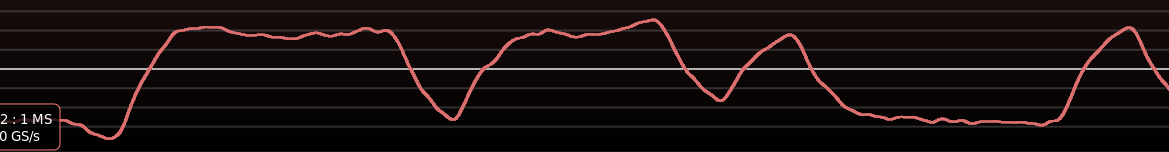
\includegraphics[width=10cm]{images/sparse-waveform.png}
\caption{Sparse waveform at a high zoom level}
\label{sparse-waveform}
\end{figure}

\begin{figure}[H]
\centering
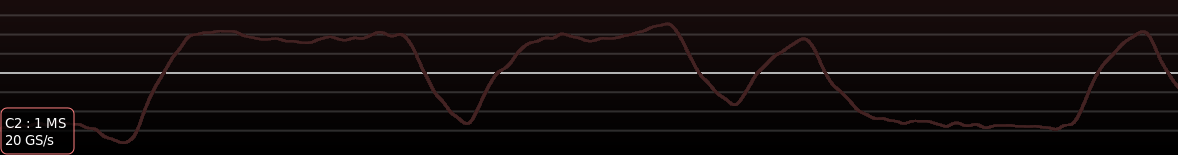
\includegraphics[width=10cm]{images/dim-waveform.png}
\caption{Dim waveform showing difficulty of seeing waveform at low opacity}
\label{dim-waveform}
\end{figure}

For example, the DVI waveform in Fig. \ref{washedout-waveform} looks like a solid white blob with a vaguely visible
outline. No fine detail can be observed other than the increased over/undershoot and random-looking edges on the
scanlines, compared to the flat appearance of the blanking period between scanlines and at the end of the frame.

When the opacity is reduced in this example, many more nuances of the signal become apparent. The high/low voltage
levels of the signal compared to the transitions between them are obvious, and the H/V sync pulses within the blanking
period show up as a slightly darker region.

\begin{figure}[H]
\centering
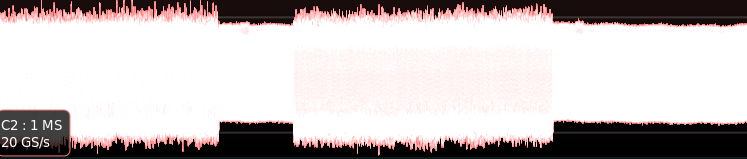
\includegraphics[width=10cm]{images/washedout-waveform.png}
\caption{Intensity-graded waveform showing washed-out appearance at high opacity}
\label{washedout-waveform}
\end{figure}

\begin{figure}[H]
\centering
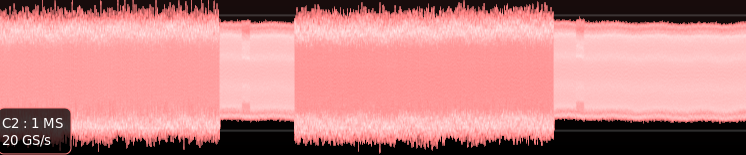
\includegraphics[width=10cm]{images/graded-waveform.png}
\caption{Intensity-graded waveform at lower opacity level}
\label{graded-waveform}
\end{figure}

As of this writing, the opacity setting is global for the entire application. Should this be changed to per waveform
group? If so, how should the group be selected and should there still be an option to make changes globally?
